\chapter{GIỚI THIỆU TỔNG QUAN}

\section{Tổng quan về an toàn và bảo mật thông tin}

\subsection{Giới thiệu}

\paragraph{}

Ngày nay với sự phát triển bùng nổ của công nghệ thông tin, hầu hết các thông tin của doanh nghiệp như chiến lược kinh doanh, các thông tin về khách hàng, nhà cung cấp, tài chính, mức lương nhân viên,…đều được lưu trữ trên hệ thống máy tính. Cùng với sự phát triển của doanh nghiệp là những đòi hỏi ngày càng cao của môi trường kinh doanh yêu cầu doanh nghiệp cần phải chia sẻ thông tin của mình cho nhiều đối tượng khác nhau qua Internet. Việc mất mát, rò rỉ thông tin có thể ảnh hưởng nghiêm trọng đến tài chính, danh tiếng của công ty và quan hệ với khách hàng. 

Hệ thống thông tin là một hệ thống bao gồm các yếu tố có quan hệ với nhau cùng làm nhiệm vụ thu thập, xử lý, lưu trữ và phân phối thông tin và dữ liệu và cung cấp một cơ chế phản hồi để đạt được một mục tiêu định trước. Các thành phần của hệ thống bao gồm phần cứng, phần mềm, mạng truyền dữ liệu, dữ liệu và con người trong hệ thống thông tin.

Các phương thức tấn công thông qua mạng ngày càng tinh vi, phức tạp có thể dẫn đến mất mát thông tin, thậm chí có thể làm sụp đổ hoàn toàn hệ thống thông tin của doanh nghiệp. Vì vậy an toàn và bảo mật thông tin là nhiệm vụ rất nặng nề và khó đoán trước được, nhưng tựu trung lại gồm ba hướng chính: 
\begin{itemize}
    \item Bảo đảm an toàn thông tin tại máy chủ 
    \item Bảo đảm an toàn cho phía máy trạm 
    \item Bảo mật thông tin trên đường truyền 
\end{itemize}

\subsection{Các mối đe dọa và thiệt hại}


\paragraph{}
Tấn công mạng là một trong những vấn đề quan trọng về an toàn và bảo mật thông tin. Đó là những nỗ lực của kẻ tấn công để truy cập vào các hệ thống mạng của một tổ chức hoặc cá nhân mà không có sự cho phép. Những tấn công mạng này có thể gây ra những thiệt hại nghiêm trọng cho các tổ chức hoặc cá nhân, bao gồm mất dữ liệu, mất tiền và thiệt hại đến danh tính.

\paragraph{}
Phần mềm độc hại: Phần mềm độc hại là một loại phần mềm được thiết kế để gây hại cho hệ thống máy tính hoặc để truy cập vào thông tin cá nhân. Các loại phần mềm độc hại bao gồm virus, phần mềm giám điệp, phần mềm mã độc và phần mềm ransonware.

\paragraph{}
Xâm nhập: Xâm nhập là quá trình xâm nhập vào hệ thống hoặc mạng của một tổ chức hoặc cá nhân mà không có sự cho phép. Các tấn công xâm nhập này có thể gây ra những thiệt hại nghiêm trọng cho các tổ chức hoặc cá nhân, bao gồm mất dữ liệu và thiệt hại đến danh tiếng. 

\paragraph{}
Lừa đảo trực tuyến: Lừa đảo trực tuyến là một hoạt động gian lận trực tuyến được thực hiện bằng cách sử dụng các kỹ thuật gian lận để lừa đảo người dùng đưa ra thông tin cá nhân hoặc tiền bạc. 

\paragraph{}
Rò rỉ dữ liệu: Rò rỉ dữ liệu là quá trình tiết lộ thông tin cá nhân hoặc thông tin nhạy cảm của một cá nhân hoặc tổ chức cho người không có quyền truy cập vào thông tin đó. Rò rỉ dữ liệu có thể gây ra những thiệt hại nghiêm trọng cho các tổ chức hoặc cá nhân.


\paragraph{}
Như vậy có thể rút ra 3 mối đe dọa chủ yếu đối với hệ thống:

\begin{itemize}
    \item Phá hoại: Kẻ thù phá hỏng thiết bị phần cứng hoặc phần mềm hoạt động trên hệ thống.
    \item Sửa đổi: Tài sản của hệ thống bị sửa đổi trái phép. Điều này thường làm cho hệ thống không hoạt động đúng chức năng của nó. Ví dụ như thay đổi mật khẩu, quyền người dùng làm họ không thể truy cập vào hệ thống để làm việc.
    \item Can thiệp: Tài sản bị truy cập bởi những người không có thẩm quyền, các truyền thông thực hiện trên hệ thống bị ngăn chặn, sửa đổi.
thống
\end{itemize}

\paragraph{}
Đe dọa đối với một hệ thống thông tin có thể đến từ nhiều nguồn khác nhau và được thực hiện bởi các đối tượng khác nhau. Có 3 loại đối tượng chính:
\begin{itemize}
	\item Các đối tượng bên trong hệ thống (insider), các đối tượng này có quyền truy cập hợp lệ đối với hệ thống.
	\item Các đối tượng bên ngoài hệ thống (hacker) thường tấn công thông qua các đường kết nối với hệ thống như Internet.
	\item Các phần mềm độc hại chạy trên hệ thống.
\end{itemize}


\subsection{Giải pháp điều khiển và kiểm soát}

\paragraph{}
Thông thường, có 3 biện pháp ngăn chặn các mối đe dọa:

\begin{itemize}
	\item Điều khiển thông qua phần mềm dựa trên các cơ chế an toàn bảo mật của hệ thống (hệ điều hành) hoặc các thuật toán mã học.
	\item Điều khiển thông qua phần cứng nhờ vào các cơ chế bảo mật, các thuật toán mã học được cứng hóa.
	\item Điều khiển thông qua chính sách của tổ chức. Tổ chức ban hành các quy định nhằm đảm bảo tính an toàn của hệ thống.
\end{itemize}

\subsection{Mục tiêu và nguyên tắc chung}

\subsubsection{Mục tiêu}

\paragraph{}
Ba mục tiêu cơ bản trong việc đảm bảo an toàn và bảo mật thông tin bao gồm: Tính bí mật, Tính toàn vẹn thông tin và Độ sẵn sàng của thông tin.
\begin{itemize}
	\item Tính bảo mật (Confidentiality): Bảo mật thông tin nghĩa là chỉ những người, máy tính được cấp phép mới có quyền truy cập và sử dụng thông tin của doanh nghiệp, hay nói cách khác, bảo mật là tránh để rò rỉ thông tin ra bên ngoài hệ thống. Những tin tặc có vô vàn cách thức để đánh cắp thông tin với mục đích xấu như giám sát hệ thống mạng của doanh nghiệp, hay Social Engineering. Vì vậy, các doanh nghiệp cần cải tiến hệ thống bảo mật thông tin (sử dụng firewall hoặc ACL, yêu cầu người dung cung cấp credential…) để tránh những việc đáng tiếc xảy ra. Tính mật của thông tin được đại diện bởi quyền READ.
	\item Tính toàn vẹn (Integrity): Đảm bảo tính toàn vẹn của thông tin nghĩa là chỉ người có thẩm quyền mới được chỉnh sửa thông tin nhưng không làm thay đổi sự chính xác của dữ liệu. Một cách phổ biến nhất để tội phạm mạng thay đổi thông tin chính là xâm nhập vào các lỗ hổng bảo mật trong hệ thống của doanh nghiệp. Tính toàn vẹn của thông tin được đại diện bởi quyền MODIFY
	\item Tính khả dụng (Availability): Có nghĩa là hệ thống lưu trữ và xử lý thông tin luôn sẵn sàng để được truy xuất ở bất cứ thời điểm nào với mục đích tránh những rủi ro về phần cứng, phần mềm, hay thậm chí tránh được hình thức tấn công từ chối dịch vụ (DoS).
	
\end{itemize}

\subsubsection{Nguyên tắc chung}

\paragraph{}
Hai nguyên tắc của bảo mật thông tin:
\begin{itemize}
	\item Việc thẩm định về bảo mật là khó, và cần tính tới tất cả tình huống tấn công có thể thực hiện.
	\item Tải sản được bảo vệ đến khi hết giá trị sử dụng hoặc hết ý nghĩa bí mật
\end{itemize}

\section{Mặt nạ dữ liệu}

\paragraph{}
\Gls{datamask} là một kỹ thuật tạo ra phiên bản dữ liệu giả nhưng giống thật của tổ chức nhằm bảo vệ thông tin nhạy cảm nhưng vẫn cung cấp các thông tin thay thế khi thông tin thực không yêu cầu. Thông tin sử dụng cho tập huấn, thử nghiệm hay kiểm thử là một vài ví dụ.

\paragraph{}
\Gls{datamask} thực hiện thay đổi giá trị của dữ liệu nhưng vẫn giữ nguyên định dạng. Mục đích của việc này là tạo ra phiên bản không thể giải mã hay dịch ngược. Có một số cách thay đổi dữ liệu như xáo trộn, hoán vị hay mã hóa.

\paragraph{}
Việc sử dụng \gls{datamask} trở nên cực kỳ quan trọng trong một số trường hợp nhờ một số lý do:

\begin{itemize}
	\item \Gls{datamask} giải quyết một số mối đe dọa quan trọng: Thất thoát, đánh cắp dữ liệu, các mối đe dọa nội bộ hay giao tiếp không an toàn với bên thứ 3.
	\item Giảm thiểu rủi ro liên quan đến sử dụng đám mây.
	\item Biến dữ liệu trở nên vô dụng đối với kẻ tấn công trong khi vẫn giữ lại các thuộc tính cho một số chức năng.
	\item Cho phép chia sẻ dữ liệu giữa các người dùng được ủy quyền như người kiểm thử và người phát triển mà không cần sử dụng dữ liệu thực.
\end{itemize}

\paragraph{}
Một số loại \gls{datamask} bao gồm:
\begin{itemize}
	\item \Gls{datamask} tĩnh: giúp tạo ra một phiên bản mới của cơ sở dữ liệu không chứa dữ liệu gốc. Thông thường, quá trình này bao gồm các bước: Sao lưu dữ liệu, xác định thông tin không cần thiết, thực hiện "đeo" mặt nạ cho dữ liệu được sao lưu.
	
	Việc sử dụng \gls{datamask} tĩnh cung cấp dữ liệu chất lượng cao cho việc phát triển và kiểm thử mà không bị lộ thông tin thực tế. Tuy nhiên, quá trình sao lưu và tạo mới tốn nhiều thời gian tùy thuộc vào độ lớn dữ liệu.
	
	\item \Gls{datamask} động: chủ yêu sử dụng chức năng phân quyền người dùng cho từng cơ sở dữ liệu hay ứng dụng. Quá trình truy cập dữ liệu được thực hiện thông qua một máy chủ trung gian. Dựa vào quyền hạn của người truy cập mà máy chủ thực hiện thay đổi dữ liệu tương ứng.
	
	\Gls{datamask} động giải quyết được vấn đề thời gian thực cho dữ liệu và thêm vào một lớp bảo mật cho cơ sở dữ liệu. Tuy nhiên dữ liệu lấy ra chất lượng không cao như phương pháp tĩnh và phụ thuộc vào máy chủ trung gian.
\end{itemize}

\paragraph{}
Các kỹ thuật \gls{datamask} đa dạng và có thể áp dụng vào các tình huống sử dụng khác nhau.
\begin{itemize}
	\item Mã hóa dữ liệu: khi dữ liệu được mã hóa, nó trở nên vô nghĩa trừ khi người đọc có khóa giải mã. Đây là một phương pháp mặt nạ kỹ thuật cao và phức tạp bởi nó yêu cầu các kỹ thuật mã hóa dữ liệu, quản lý và chia sẻ khóa mã hóa.
	\item Xáo trộn dữ liệu: các ký tự được xáo trộn ngẫu nhiên thay thế cho dữ liệu gốc. Đây là một phương pháp dễ thực hiện nhưng chỉ có thể áp dụng cho một số loại dữ liệu cụ thể và kém bảo mật.
	\item Thay thế dữ liệu: dữ liệu được thay thế bởi dữ liệu cố định khi truy cập bởi người dùng không được ủy quyền. Phương pháp này khiến dữ liệu trở nên kém hữu ích cho việc phát triển và kiểm thử.
	\item Làm giả dữ liệu: dữ liệu được thay thể bởi dữ liệu giả nhưng giống thật được tạo ra ngẫu nhiên.
\end{itemize}

\paragraph{}
Đối với kỹ thuật \gls{encrypt} dữ liệu, ngoài việc ẩn đi dữ liệu gốc, dữ liệu \gls{encrypt} có thể được khôi phục trực tiếp đối với người dùng có khóa \gls{decrypt}. Vì vậy khóa \gls{decrypt} cần được quản lý riêng.

\section{Mã hóa dữ liệu}

\paragraph{}
\Gls{encrypt} được coi là phương pháp bảo vệ hiệu quả giúp đảm bảo bảo mật và sự riêng tư của dữ liệu. Phương pháp này cung cấp tính bảo mật trong bộ ba mục tiêu Bảo mật-Toàn vẹn-Sẵn sàng. Nếu dữ liệu được \gls{encrypt} bị mất hay truy cập không được phép, nó vẫn luôn được bảo vệ. Vì vậy, nó có thể được sử dụng để truyền dữ liệu qua kênh công khai nay được dùng \gls{encrypt} dữ liệu trước khi lưu vào cơ sở dữ liệu.

\paragraph{}
Hai phương pháp mã hóa được sử dụng là mã hóa đối xứng và mã hóa không đối xứng:
\begin{itemize}
	\item \Gls{symmetric cipher} là phương pháp mã hóa sử dụng chung một khóa bí mật. Một số thuật toán mã hóa bao gồm \gls{aes}, \gls{3des}, \gls{chacha}, ...
	\item \Gls{asymmetric cipher} sử dụng 2 khóa độc lập: khóa công khai và khóa bí mật. Khi dữ liệu được mã hóa bởi bởi khóa công khai, chỉ có khóa bí mật tương ứng mới có thể giải mã. \gls{rsa} là thuật toán lâu đời và nổi tiếng nhất cho phương pháp mã hóa này. Ngoài ra các thuật toán khác như \gls{elgamal encryption} cũng có các ưu điểm riêng.
\end{itemize}

\section{Cơ sở dữ liệu SQLite}

\paragraph{}
SQLite là một \gls{dbms} quan hệ tương tự như MySQL, ... Đặc điểm nổi bật của SQLite so với các \gls{dbms} khác là gọn, nhẹ, đơn giản, đặt biệt không cần mô hình server-client, không cần cài đặt, cấu hình hay khởi động nên không có khái niệm user, password hay quyền hạn trong SQLite Database. Dữ liệu cũng được lưu ở một file duy nhất.

\paragraph{}
SQLite thường không được sử dụng với các hệ thống lớn nhưng với những hệ thống ở quy mô vùa và nhỏ thì SQLite không thua các \gls{dbms} khác về chức năng hay tốc độ. Vì không cần cài đặt hay cấu hình nên SQLite được sử dụng nhiều trong việc phát triển, thử nghiệm … vì tránh được những rắc rối trong quá trình cài đặt.

\paragraph{}
Do được lưu trữ trực tiếp trên một file duy nhất, nếu không quản lý tốt trong hệ thống file, dữ liệu có thể bị lộ một cách dễ dàng. Một cách khác giúp bảo vệ dữ liệu trong SQLite là áp dụng mã hóa dưới dạng mặt nạ dữ liệu cho các bảng bên trong cơ sở dữ liệu.

\paragraph{}
SQLite có một hệ thống kiểu dữ liệu đơn giản bao gồm 5 kiểu:
\begin{itemize}
	\item NULL: giá trị NULL.
	\item Integer: giá trị số nguyên có độ dài 8, 16, 32 hay 64 bit tùy thuộc vào giá trị.
	\item Float: giá trị số thực 64 bit.
	\item Text: giá trị kiểu chuỗi Unicode.
	\item Blob: giá trị kiểu blob có thể chứa số lượng byte không biết trước. Đây là kiểu dữ liệu đa dụng nhất có thể lưu trữ toàn bộ các kiểu dữ liệu còn lại hoặc lưu trữ dữ liệu đã được mã hóa.
\end{itemize}

\section{Hệ mã dòng có xác thực \Gls{chachapoly}}

\paragraph{}
\Gls{chachapoly} là hệ mã dòng có kiến trúc mã hóa với dữ liệu liên kết (Authenticated Encryption with Additional Data - AEAD) cung cấp tính bí mật và xác thực nguồn gốc dữ liệu truyền nhận trên kênh liên lạc.
\Gls{chachapoly} có kiến trúc bao gồm hai thành phần chính là thuật toán mã dòng ChaCha20 và cơ chế xác thực Poly1305 của cùng tác giả là D.J. Berstein.

\begin{figure}[H]
	\centering
	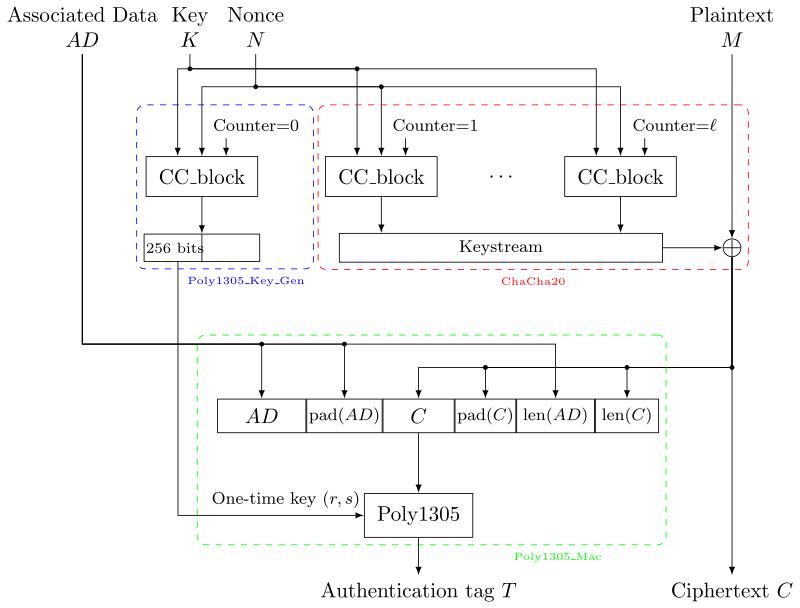
\includegraphics[width=0.8\textwidth]{images/ChaCha20-Poly1305_Encryption.png}
	\caption{Sơ đồ khối hệ mã dòng có xác thực \Gls{chachapoly}}
\end{figure}

\subsection{Hệ mã dòng ChaCha}

\paragraph{}
ChaCha có trạng thái khởi tạo rộng 64 byte (512bit) bao gồm lần lượt 16 byte cố đinh $"expand\ 32-byte\ k"$, \gls{key} độ dài 32 byte, 8 byte counter và 8 byte vector khởi tạo. Trạng thái này chia thành 16 khối 4 byte trên ma trận 4x4 để đưa vào \gls{quarter}-\gls{round function}.

\begin{table}[h]
	\caption{Trạng thái khởi tạo của thuật toán ChaCha}
	\centering
	\begin{tabular}{|c|c|c|c|}
		\hline
		"expa" & "nd 3" & "2-by" & "te k"\\
		\hline
		key[0..4] &key[4..8] &key[8..12] &key[12..16] \\
		\hline
		key[16..20] &key[20..24] &key[24..28] &key[28..32] \\
		\hline
		counter[0..4] & counter[4..8] & nonce[0..4] & nonce[4..8]\\
		\hline
	\end{tabular}

\end{table}

\paragraph{}
Từng bộ trong 4 bộ 4 byte lần lượt được đưa vào \gls{quarter}-\gls{round function} tạo lên một vòng. Đối với vòng lẻ, lần lượt 4 khối trên từng cột của ma trận trạng thái được đưa vào \gls{quarter}-\gls{round function}, đối vòng chẵn, lần lượt 4 khối trên 4 hàng của ma trận trạng thái được đưa vào \gls{quarter}-\gls{round function}.

\begin{figure}[h]
	\centering
	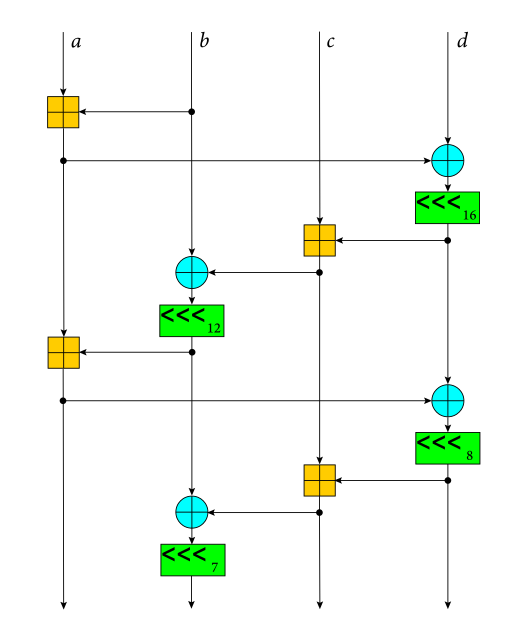
\includegraphics[width=0.5\textwidth]{images/ChaCha_Cipher_Quarter_Round_Function.png}
	\caption{\Gls{quarter}-\gls{round function} của thuật toán ChaCha}
\end{figure}

\paragraph{}
Tên của từng thuật toán ChaCha ứng với số vòng được áp dụng như ChaCha8 thực hiện 8 vòng, ChaCha20 thực hiện 20 vòng.

\paragraph{}
Sau khi qua các vòng, ma trận trạng thái được sử dụng để cộng modulo-2 với tối đa 64 byte bản rõ tạo thành 64 byte bản mã. Nếu độ dài bản rõ nhiều hơn 64 byte, giá trị counter trong trạng thái khởi tạo được cộng thêm 1 và thực hiện qua các vòng để áp dụng cho các khối tối đa 64 byte tiếp theo.

\paragraph{}
Quá trình \gls{decrypt} từ bản mã thành bản rõ được thực hiện giống quá trình \gls{encrypt} do việc biến đổi chỉ dựa trên phép cộng modulo-2.

\subsection{Cơ chế xác thực Poly1305}

\paragraph{}
\Gls{poly1305} là cơ chế xác thực thông báo với đầu vào khóa 256 bit và thông báo có độ dài không cố định. Đầu ra là một thẻ xác thực độ dài 128 bit được sử dụng bởi bên nhận nhằm xác thực nguồn thông báo.

\paragraph{}
\Gls{key} đầu vào được chia thành 2 phần gọi là $r$ và $s$ có độ dài 128 bit. Cặp $(r, s)$ phải là duy nhất và không thể đoán cho mỗi lần gọi. $r$ cần được xử lý bằng cách XOR với 0x0ffffffc0ffffffc0ffffffc0fffffff. 

\paragraph{}
Thông báo đầu vào được chia thành các khối 16 byte, khối cuối cùng có thể ngắn hơn được thêm các bit 0. Các khối 16 byte này được thêm vào 1 byte có giá trị 0x01 thành 17 byte. Các phép tính được thực hiện trên các khối này với r trên trường Z () để tạo một bộ tích lũy ACC như trong hình \ref{fig:polycalc}.

\begin{figure}[h]
	\centering
	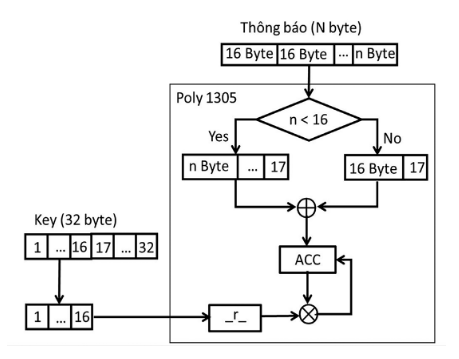
\includegraphics[width=0.8\textwidth]{images/poly1305.png}
	\caption{Quá trình tính toán của cơ chế Poly1305}
	\label{fig:polycalc}
\end{figure}

Cuối cùng giá trị s được thêm vào bộ tích lũy và 128 bit được lấy ra làm thẻ xác thực. Xem hình \ref{fig:polytag}.

\begin{figure}[h]
	\centering
	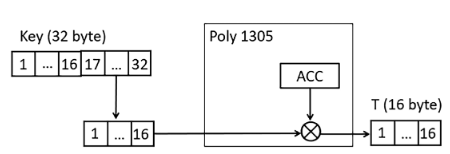
\includegraphics[width=0.8\textwidth]{images/poly.png}
	\caption{Tính toán thẻ xác thực trong Poly1305}
	\label{fig:polytag}
\end{figure}

\section{Hàm băm BLAKE2s}

\paragraph{}
BLAKE là \gls{hash function} mật mã dựa trên mã dòng \gls{chacha} của Daniel J. Bernstein nhưng một bản sao hoán vị của khối đầu vào được XOR với các hằng số vòng được thêm vào trước mỗi bước vòng của \gls{chacha}.

ChaCha sử dụng ma trận trạng thái kích thước $4x4$ word. BLAKE liên tục kết hợp 8 word giá trị băm với 16 word giá trị thông báo, cắt bớt giá trị trả về của ChaCha để lấy giá trị \gls{hash} tiếp theo. BLAKE-256 sử dụng word độ dài 32 bit và thu được 256 bit \gls{hash}. 

BLAKE2 được phát triển dựa trên BLAKE bằng cách tinh giản BLAKE và giảm số vòng từ 16 xuống 12 đối với BLAKE2b và từ 14 xuống 10 đối với BLAKE2s.

BLAKE2s là biến thể BLAKE2 được phát triển từ BLAKE-256, có độ dài đầu ra 256 bit.

\section{Trao đổi khóa Diffie-Hellman và Elliptic-curve Diffie-Hellman}

\subsection{Trao đổi khóa Diffie-Hellman}

\paragraph{}
\Gls{dh} là một phương pháp trao đổi khóa được phát minh sớm nhất trong mật mã học. Phương pháp \gls{dh} cho phép 2 hay nhiều bên thiết lập một khóa bí mật chung để mã hóa dữ liệu sử dụng trên kênh không an toàn mà không cần có sự thỏa thuận trước về khóa bí mật giữa hai bên. \Gls{key} bí mật được tạo ra có thể sử dụng để mã hóa dữ liệu với phương pháp \gls{asymmetric cipher}.

Quá trình thiết lập khóa được mô tả như sau:
\begin{enumerate}
	\item Hai bên sử dụng chung một nhóm cyclic hữu hạn $G$, một phần tử sinh $g$ thuộc $G$ và số nguyên số $p$.
	\item Alice chọn số $a$ ngẫu nhiên và gửi $g^a$ mod $p$ cho Bob.
	\item Bob tương tự chọn số $b$ ngẫu nhiên và gửi $g^b$ mod $p$ cho Alice.
	\item Alice tính $(g^b)^a$ mod $p$.
	\item Bob tính $(g^a)^b$ mod $p$.
\end{enumerate}

\paragraph{}
Như vậy sau quá trình tính toán, hai bên có chung giá trị bí mật chung $g^{ab}$ mod $p$. Và có thể được sử dụng để \gls{encrypt} hoặc tạo khóa \gls{encrypt}. Việc tính ra $g^{ab}$ mod $p$ từ các giá trị $g$, $p$, $g^a$, $g^b$ được mô tả dưới dạng bài toán tính logarit rời rạc và được chứng minh là bài toán khó ngay cả đối với siêu máy tính.

\paragraph{}
Ngoài chức năng trao đổi khóa, \gls{dh} còn được sử dụng như một phần của hạ tầng khóa công khai. Khi đó, khóa công khai của A là ($g^a$ mod $p$, $g$, $p$). Để mã hóa công khai cho A, B chọn số $b$ ngẫu nhiên và gửi $g^b$ mod $p$ cũng thông điệp được mã hóa bởi \gls{key} $(g^a)^b$ mod $p$. Do $a$ được giữ bí mật, chỉ A có thể giải mã được thông điệp.

\subsection{Mật mã đường cong Elliptic}

\paragraph{}
\gls{ecc} là một trong những loại hiện đại, mạnh nhất hiện nay, cung cấp hiệu năng cao và an toàn hơn so với thế hệ đầu tiên \gls{rsa}. Với độ dài 256 bit, khóa hệ mật trên đường cong elliptic có độ bảo mật tương đương khóa RSA độ dài 3248 bit.

\paragraph{}
Đường cong elliptic được biểu diễn dưới dạng $y^2=x^3+ax+b$. \gls{ecc} hoạt động dựa trên dựa trên tính chất đường thẳng bất kỳ cắt đường cong elliptic tại nhiều nhất 3 điểm.

\begin{figure}[h]
	\centering
	\begin{subfigure}[b]{0.4\textwidth}
		\centering
		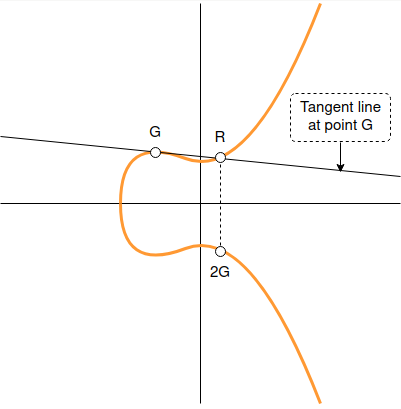
\includegraphics[width=\textwidth]{images/Point_doubling.png}
		\caption{Nhân đôi điểm}
		\label{fig:poindoubling}
	\end{subfigure}
	\begin{subfigure}[b]{0.4\textwidth}
		\centering
		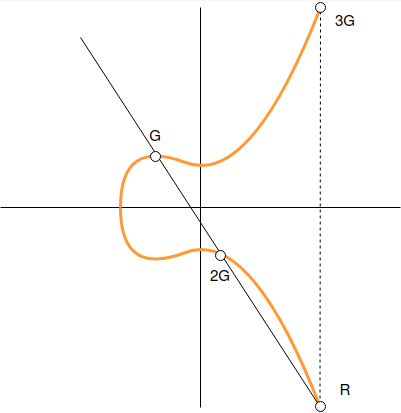
\includegraphics[width=\textwidth]{images/Point_addition.png}
		\caption{Cộng hai điểm}
		\label{fig:poinadditioning}
	\end{subfigure}

	\caption{Hai thao tác trên đường cong elliptic}

\end{figure}

\paragraph{}
Nhân đôi điểm được sử dụng khi có 1 điểm A ban đầu. Đường tiếp tuyến với đường cong tại A sẽ cắt đường cong tại B. Đường thẳng song song với trục tung cắt đường cong tại điểm là kết quả của phép toán. Trong hình \ref{fig:poindoubling} ta có điểm ban đầu G và kết quả 2G.

\paragraph{}
Cộng 2 điểm được thực hiện với 2 điểm đầu vào. Đường thẳng đi qua 2 điểm cắt đường thẳng tại điểm thứ 3. Đường thằng song song với trục tung đi qua điểm này cắt đường cong tại điểm thứ 2 là kết quả của phép toán. Hình \ref{fig:poinadditioning} mô tả phép cộng 2 điểm G và 2G cho kết quả 3G.

\paragraph{}
Các tham số của ECC có dạng ($p$, $a$, $b$, $G$, $n$, $h$):
\begin{itemize}
	\item $a$, $b$ là tham số đường cong elliptic.
	\item Số nguyên tố $p$ lớn giới hạn kích thước trường giá trị.
	\item Điểm khởi đầu $G$
	\item Số điểm $n$ trên đường cong
	\item Số nhóm cyclic $h$ của đường cong. Một số đường cong có 1 nhóm, một số khác có nhiều hơn 1 nhóm.
\end{itemize}

\subsection{Trao đổi khóa Diffie-Hellman trên đường cong elliptic}

\paragraph{}
Thay vì sử dụng phép lũy thừa như \gls{dh}, \gls{ecdh} sử dụng phép nhân trong \gls{ecc} để sinh khóa.

\paragraph{}
\gls{ecdh} thực hiện 2 bước thỏa thuận khóa: tạo \gls{key} và tính toán giá trị bí mật chung. 

\paragraph{}
Tham số bí mật là số $n$ ngẫu nhiên với $n \in 1..n_0$. Tham số công khai được tính $P = nG$ với $n$ là tham số bí mật, $G$ là điểm sinh, $P$ là tham số công khai.

\paragraph{}
Giá trị bí mật được tính bằng $S = P_1* n_2 = P_2*n_1 = n_1 * n_2 * G = n_2 * n_1 * G$

